
%(BEGIN_QUESTION)
% Copyright 2007, Tony R. Kuphaldt, released under the Creative Commons Attribution License (v 1.0)
% This means you may do almost anything with this work of mine, so long as you give me proper credit

Some serial network standards (such as EIA/TIA-232) use {\it single-ended} driver circuits to generate the communication signals.  An example is shown here:

$$\includegraphics[width=15.5cm]{i02191x01.eps}$$

Other serial network standards (such as EIA/TIA-422 and EIA/TIA-485) use {\it differential} driver circuits to generate the communication signals.  An example appears below:

$$\includegraphics[width=15.5cm]{i02191x02.eps}$$

At first the differential design may appear less attractive because it requires one more wire.  However, there are significant operational advantages to differential signaling over single-ended signaling.  Explain why differential signaling is preferred, especially for industrial (high electrical noise) and high-speed (high signal frequency) applications.

\underbar{file i02191}
%(END_QUESTION)





%(BEGIN_ANSWER)

The answer really hinges on how the voltage signals represent digital data.  In the single-ended scheme, all signal voltages make reference to the same ground wire:

$$\includegraphics[width=15.5cm]{i02191x03.eps}$$

\vskip 10pt

In the differential scheme, each transmission path is electrically independent:

$$\includegraphics[width=15.5cm]{i02191x04.eps}$$

\vskip 10pt

Since single-ended signaling depends on a {\it common-mode voltage} for data representation, common-mode noise has a great effect on data integrity.  By contrast, differential signaling relies on {\it differential voltage} only, and so common-mode noise voltage is ignored.  

Also, common-mode signaling invites capacitive coupling between the two data lines, which may lead to data corruption at high frequencies.  Differential signaling, due to the lack of a common ground between the two data pathways, is less prone to ``coupling.''

\vskip 10pt

Differential signaling is more tolerant to noise, allowing lower signal voltage levels.  The lower voltage levels in turn allow faster communication rates due to slew rate limiting of the driver circuits.

%(END_ANSWER)





%(BEGIN_NOTES)


%INDEX% Networking, serial: single-ended versus differential signaling

%(END_NOTES)


